\documentclass[tikz,border=8pt]{standalone}
% Shared look for every TikZ diagram. Load with % Shared look for every TikZ diagram. Load with % Shared look for every TikZ diagram. Load with \input{../../tools/tikz-style.tex}
\usepackage[T1]{fontenc}
\usepackage{lmodern}
\renewcommand{\sfdefault}{lmr}  % diagrams use the same serif as the text
\usetikzlibrary{arrows.meta, positioning, shapes.geometric, calc, fit, backgrounds}
\definecolor{cblue}{HTML}{4C78A8}
\definecolor{corange}{HTML}{F58518}
\definecolor{cgreen}{HTML}{54A24B}
\definecolor{cred}{HTML}{E45756}
\definecolor{cpurple}{HTML}{B279A2}
\definecolor{cgrey}{HTML}{6B6B6B}
\tikzset{
  every picture/.style={font=\sffamily, line width=1.2pt},
  box/.style={draw=#1, fill=#1!12, rounded corners=4pt, align=center, inner sep=7pt, minimum height=1.1cm},
  box/.default=cgrey,
  arrow/.style={-{Stealth[length=3mm]}, draw=cgrey, line width=1.4pt},
  title/.style={font=\sffamily\bfseries\Large},
  note/.style={font=\sffamily\small, text=cgrey, align=center},
}
\AtBeginDocument{\hyphenpenalty=10000 \exhyphenpenalty=10000}

\usepackage[T1]{fontenc}
\usepackage{lmodern}
\renewcommand{\sfdefault}{lmr}  % diagrams use the same serif as the text
\usetikzlibrary{arrows.meta, positioning, shapes.geometric, calc, fit, backgrounds}
\definecolor{cblue}{HTML}{4C78A8}
\definecolor{corange}{HTML}{F58518}
\definecolor{cgreen}{HTML}{54A24B}
\definecolor{cred}{HTML}{E45756}
\definecolor{cpurple}{HTML}{B279A2}
\definecolor{cgrey}{HTML}{6B6B6B}
\tikzset{
  every picture/.style={font=\sffamily, line width=1.2pt},
  box/.style={draw=#1, fill=#1!12, rounded corners=4pt, align=center, inner sep=7pt, minimum height=1.1cm},
  box/.default=cgrey,
  arrow/.style={-{Stealth[length=3mm]}, draw=cgrey, line width=1.4pt},
  title/.style={font=\sffamily\bfseries\Large},
  note/.style={font=\sffamily\small, text=cgrey, align=center},
}
\AtBeginDocument{\hyphenpenalty=10000 \exhyphenpenalty=10000}

\usepackage[T1]{fontenc}
\usepackage{lmodern}
\renewcommand{\sfdefault}{lmr}  % diagrams use the same serif as the text
\usetikzlibrary{arrows.meta, positioning, shapes.geometric, calc, fit, backgrounds}
\definecolor{cblue}{HTML}{4C78A8}
\definecolor{corange}{HTML}{F58518}
\definecolor{cgreen}{HTML}{54A24B}
\definecolor{cred}{HTML}{E45756}
\definecolor{cpurple}{HTML}{B279A2}
\definecolor{cgrey}{HTML}{6B6B6B}
\tikzset{
  every picture/.style={font=\sffamily, line width=1.2pt},
  box/.style={draw=#1, fill=#1!12, rounded corners=4pt, align=center, inner sep=7pt, minimum height=1.1cm},
  box/.default=cgrey,
  arrow/.style={-{Stealth[length=3mm]}, draw=cgrey, line width=1.4pt},
  title/.style={font=\sffamily\bfseries\Large},
  note/.style={font=\sffamily\small, text=cgrey, align=center},
}
\AtBeginDocument{\hyphenpenalty=10000 \exhyphenpenalty=10000}

\begin{document}
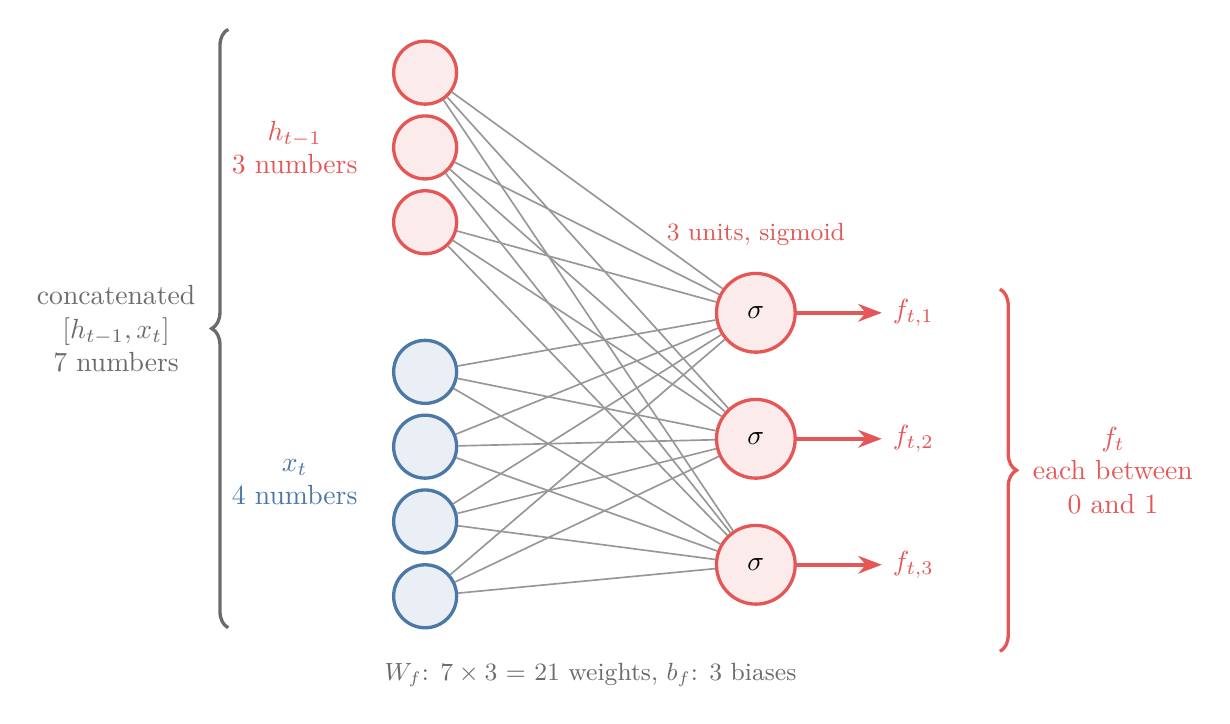
\begin{tikzpicture}[neuron/.style={circle, draw=#1, fill=#1!12, minimum size=0.8cm, line width=1.2pt}]
  \foreach \k in {1,2,3} \node[neuron=cred] (h\k) at (0,4.4-0.95*\k) {};
  \foreach \k in {1,2,3,4} \node[neuron=cblue] (x\k) at (0,0.6-0.95*\k) {};
  \node[left=0.3cm of h2, text=cred, align=center] {$h_{t-1}$\\3 numbers};
  \node[left=0.3cm of x2, yshift=-0.45cm, text=cblue, align=center] {$x_t$\\4 numbers};
  \draw[decorate, decoration={brace, amplitude=6pt, mirror}, cgrey] (-2.5,4.0) -- (-2.5,-3.6) node[midway, left=8pt, text=cgrey, align=center] {concatenated\\$[h_{t-1}, x_t]$\\7 numbers};
  \foreach \j in {1,2,3} \node[neuron=cred, minimum size=1.0cm] (f\j) at (4.2,2.0-1.6*\j) {$\sigma$};
  \foreach \a in {h1,h2,h3,x1,x2,x3,x4} \foreach \j in {1,2,3} \draw[cgrey!70, line width=0.6pt] (\a) -- (f\j);
  \node[note, text=cred] at (4.2,1.4) {3 units, sigmoid};
  \node[note] at (2.1,-4.2) {$W_f$: $7 \times 3$ = 21 weights, $b_f$: 3 biases};
  \foreach \j in {1,2,3} \draw[arrow, draw=cred] (f\j) -- ++(1.6,0) node[right, text=cred] {$f_{t,\j}$};
  \draw[decorate, decoration={brace, amplitude=6pt}, cred] (7.3,0.7) -- (7.3,-3.9) node[midway, right=8pt, text=cred, align=center] {$f_t$\\each between\\0 and 1};
\end{tikzpicture}
\end{document}
